\documentclass[11pt]{article}
\usepackage[T1]{fontenc}
\usepackage[utf8]{inputenc}
\usepackage[margin=1in]{geometry}
\usepackage{amsmath,amssymb,booktabs,graphicx,hyperref,array}
\setlength{\emergencystretch}{2em}
\hypersetup{colorlinks=true,linkcolor=blue,citecolor=blue,urlcolor=blue}
\title{A Dose-Dependent Crossover in Transcoder Fidelity:\\Held-Out Prediction and Residual Geometry}
\author{Author information to be supplied}
\date{November 4, 2026 --- private working manuscript, version 16}
\begin{document}
\maketitle
\begin{abstract}
Local response fidelity and useful finite-intervention prediction can diverge. A public Gemma-270M transcoder has 10.11\% relative RMS pronoun-readout error at a full donor patch on fresh lexical blocks, while native-vector Taylor is better at small dose. A second Gemma artifact repeats the Taylor--transcoder ranking crossover but has poor full-patch accuracy, separating relative ranking from usefulness. Residual substitutions, selected-mask interventions and a fresh fixed-norm direction diagnostic characterize bounded properties of the first artifact's predictions. Their dependence on intervention construction, overlapping controls and eligible contexts constrains the explanation. A negative Qwen component test further bounds transfer. The central result is artifact-specific finite-effect usefulness within a dose-dependent fidelity curve.
\end{abstract}

\section{Introduction}
A transcoder approximates a native branch's computation using sparse features. Its value as an intervention model depends on how accurately changes in its prediction reproduce the native downstream effect. We study that accuracy across intervention strengths, contrasting the fixed public transcoder with native-vector Taylor and FIT-trained predictors.

The central observation is a dose-dependent ranking crossover on Gemma-3-270M layer 15. At small dose, native Taylor has much lower downstream readout error; at a full donor patch, the transcoder has lower error than Taylor, ridge and the FIT class mean, including on a predeclared transfer template. The artifact and regime were selected historically, followed by a new frozen lexical TEST. A second public Gemma artifact repeats the crossover but loses to zero change and ridge at the full patch. This distinction makes useful accuracy, rather than superiority to one approximation, the substantive result.

We then examine prediction-error geometry. Endpoint reconstruction errors can cancel in a difference, while the remaining vector residual is filtered by a nonlinear native suffix. Same-dose residual substitutions and selected-mask interventions probe these two stages. A subsequent fixed-norm diagnostic gives a large selected-versus-control prediction-damage contrast on exposed and fresh lexical blocks. The controls overlap and sometimes produce identical directions; their frozen weights are retained. Changed-context and object-readout coverage provide further limits.

Table~\ref{tab:scope} separates the fresh predictions, exposed-data diagnostics and shared-cohort Qwen boundary. The supplementary report preserves all earlier hypotheses, failed forecasts, complete dose grids, detailed protocols and forensic checks.

\begin{table}[ht]\centering\scriptsize
\setlength{\tabcolsep}{4pt}
\begin{tabular}{>{\raggedright\arraybackslash}p{.20\textwidth}>{\raggedright\arraybackslash}p{.34\textwidth}>{\raggedright\arraybackslash}p{.37\textwidth}}\toprule
Study & Sample and reuse & Reporting scope\\\midrule
Gemma-270M main & 256 fresh name-pair blocks; so/when and transfer share names; 1,536 contexts & Fixed six-dose/two-operator TEST; descriptive finite-corpus errors. Separate qualified intervals cover 12 full-dose TC metrics.\\[3pt]
Gemma-1B replication & 256 additional disjoint blocks; six doses, full donor operator & Frozen FIT/protocol; historically exposed artifact; nominal block intervals.\\[3pt]
Residual/mask tests & 32 exposed 270M blocks, indices 16--47; 768 dependent conditions & Posthoc whole-residual substitutions and FIT-selected masks. Earlier 16-block construction is separately retained.\\[3pt]
Strength/direction tests & Cached FIT32; then exposed TEST32; then fresh32 blocks & Failed unscaled matching; fixed-norm diagnostic; fresh result is descriptive. Transfer 45/64 contexts; object 12/64.\\[3pt]
Qwen boundary & 256 shared companion blocks; 4,096 unit-dose native/ridge margins adopted & Descriptive CLT-component dose curve; shared lexical cohort and selected outputs.\\\bottomrule
\end{tabular}
\caption{Evidence map. Lexical blocks are the sampling units. Repeated templates, doses, fits and control groups retain their dependence. Each stage has separate independent scientific completion receipts.}\label{tab:scope}
\end{table}

\section{Related work}
Transcoder circuits, sparse-feature interventions and their validation are established research areas~\cite{dunefsky2024,ameisen2025}. JumpReLU's discontinuous threshold~\cite{rajamanoharan2024} and Jacobian-aware approaches~\cite{farnik2025,shabalin2026} motivate measuring both local and finite responses. Formal replacement-discrepancy bounds~\cite{ladner2026} address a neighboring question over activation sets; our outcome is baseline-subtracted native readout-effect prediction.

Strength controls can change sparse-code intervention rankings~\cite{zhang2026}. Luo et al.~\cite{luo2026} additionally match surface and basis when comparing sparse and dense safety interventions. Their results place our fixed-norm direction controls in context: output-norm matching answers a specified comparison while leaving other properties of the interventions unequal. Deshpande~\cite{deshpande2026} studies which refitted readouts survive sparse compression, complementing our native-suffix measurements of intervention deltas.

Guo et al.~\cite{guo2026} define intervention attribution as an average edit--gradient product and evaluate attribution-selected feature sets. This is a direct precedent for any proposed gradient-based selection or explanation of the directions studied here. Existing attribution-patching work also treats finite-dose nonlinear error~\cite{zhangwang2026}. Our Taylor comparator instead linearizes the native branch vector and then runs the exact nonlinear suffix. Baz\'an S\'anchez~\cite{bazan2026} predicts complete feature removal from a measured midpoint intervention inside transcoder replacements; our public TC predictions use target-free inputs and are evaluated against native branch interventions. These distinctions identify the empirical estimand and its closest precedents.

\section{Prediction target and experimental design}
\subsection{Native changes and downstream readout}
Let $f(z)$ be the native branch, including its documented normalization, and $T(z)$ the fixed transcoder. Recipient input $z$, donor difference $d=z_d-z$ and a unit FIT class-mean direction $w$ define
\[
 \delta_{full}=cd,\qquad \delta_{proj}=c(d^\top w)w,
 \quad c\in\{.05,.1,.25,.5,1,2\}.
\]
The native target and main predictions are
\[
 \Delta_N=f(z+\delta)-f(z),\quad
 \Delta_T=T(z+\delta)-T(z),\quad
 \Delta_J=J_f(z)\delta.
\]
Each predicted vector is added to the recipient's native branch output and propagated through the exact native suffix. In Gemma-270M this includes dynamic attention in layers 16 and 17. Native Taylor is therefore a branch-vector JVP followed by nonlinear downstream evaluation. The tested boundary is the post-feedforward-normalized layer-15 output at the final token.

If $m_N$ is the native intervention's change in she-minus-he logit margin and $m_v$ its prediction, the relative RMS error is
\[
 \epsilon_v=\sqrt{\frac{\sum_i(m_{v,i}-m_{N,i})^2}{\sum_i m_{N,i}^2}}.
\]
Zero change gives 100\%. Energies are pooled before the ratio and square root. Absolute RMS and native signal RMS accompany the relative errors. Within a fixed cell all methods share the denominator, preserving their absolute-error ranking. The full and projected operators can have unequal edit norms at the same coefficient $c$.

\subsection{Fixed artifacts, FIT and fresh lexical cohorts}
The main artifact is the public medium Gemma-3-270M layer-15 transcoder, with no affine skip. The native model has no final-logit softcap. Native runtime is FP32; exact-prefix/suffix parity was separately qualified. Vector-only FIT uses 32 name-pair blocks and 128 natural states across so/when to fix $w$, class-cell means and ridge baselines (centered intercept, global input RMS, $\lambda=.01$). Frozen mask keeps the baseline TC feature mask fixed. These baselines use no TEST deltas or readout labels.

A separate 32-block PILOT precedes the main TEST: 256 disjoint name-pair blocks, two sides and three templates, giving 1,536 recipient documents. The primary mixture pools so/when; the third form is predeclared transfer. The original report includes 288 method/dose/operator/template summaries and 18,432 records. The second artifact is the locally available Gemma-3-1B layer-22 medium 16k, $L_0=60$, no-affine transcoder, chosen by an availability/depth rule before new outcomes. It uses 32 fresh FIT and 256 further disjoint TEST blocks, the full donor operator and all six doses, scored through native layers 23--25 and the final head.

Both artifacts have historical exploratory exposure. New lexical splits and fixed acquisition rules give prospective conditional tests of the selected artifacts. Public-TC training resources and FIT-native-label costs differ and are recorded separately. Full checkpoint identities, model/TC revisions, hooks, budgets and immutable review bindings are retained in the supplement.

\subsection{Inference and acquisition chronology}
The primary Gemma-270M TEST is a fixed-$N$ descriptive study. Its originally proposed hypothesis family failed qualification in two of 54 synthetic scenarios; the original family therefore supplies no population rejection claims. A separate pre-TEST interval amendment qualified paired studentized log-RMS max-statistic intervals for 12 full-dose TC metrics. Their construction confidence is 99\%, with finite-scenario qualification. Transfer and other dose/comparator cells remain descriptive.

The Gemma-1B follow-up reports nominal 95\% intervals from the saved 1,999-draw block bootstrap, conditional on fixed FIT objects. Exposed-data residual diagnostics and the fresh equal-norm follow-up have their own descriptive scope. Block means or pooled block energies preserve dependence across sides/templates; five alternative feature groups do not create five independent samples. All manuscript values come from completed, independently reviewed scientific stages.

\section{Dose crossover and useful finite accuracy}
\subsection{Gemma-270M: Taylor wins locally, TC at the full patch}
Table~\ref{tab:main} shows the central reversal. At the full donor patch, the transcoder has 10.11\% relative RMS error versus Taylor's 129.96\% and ridge's 28.05\%. At dose .05, TC error is 117.46\%, versus Taylor's 12.10\%. Projected full-patch prediction shows the same favorable TC regime. The complete curves are in Figure~\ref{fig:dose} and the supplementary dose grids.

\begin{table}[ht]\centering\small
\begin{tabular}{lrrr}\toprule Predictor & Full $c=1$ & Projected $c=1$ & Full $c=.05$\\\midrule
Transcoder & 10.11 & 11.07 & 117.46\\
Native Taylor & 129.96 & 128.09 & 12.10\\
Frozen mask & 108.35 & 108.06 & 110.16\\
FIT class-cell mean & 57.73 & 57.94 & 127.72\\
FIT ridge & 28.05 & 32.53 & 173.81\\
Zero change & 100.00 & 100.00 & 100.00\\\bottomrule\end{tabular}
\caption{Gemma-270M TEST relative RMS margin-prediction error, percent. Each column pools 256 blocks with equal sides and so/when weights. These are descriptive finite-corpus summaries; the separately qualified full-dose TC intervals are reported in the text.}\label{tab:main}
\end{table}

The reversal holds in absolute error as well. At dose .05, TC and Taylor RMS errors are .06030 and .00621 logits. At dose 1, TC, Taylor and ridge errors are .34963, 4.49225 and .96966. TC absolute error increases, while native signal RMS grows from .05134 to 3.45655 logits. This explains the decrease in its relative error across doses without attributing the cross-method ranking to different denominators.

On the predeclared transfer template at full dose, TC error is 16.28\% full and 17.59\% projected, compared with Taylor's 115.44\%/110.05\% and ridge's 40.10\%/35.83\%. At dose .05, transfer TC errors are 97.78\%/97.73\%. The full-patch favorable regime therefore extends to this template with weaker accuracy than on the main mixture.

The qualified main-mixture full-dose TC intervals are [8.99\%,11.38\%] for full edits and [9.78\%,12.53\%] for projected edits. Eleven of twelve desired interval-width targets are met. Projected/when has halfwidth 2.431 percentage points, exceeding its 2-point target. Method qualification and actual precision attainment are reported separately.

\begin{figure}[ht]\centering
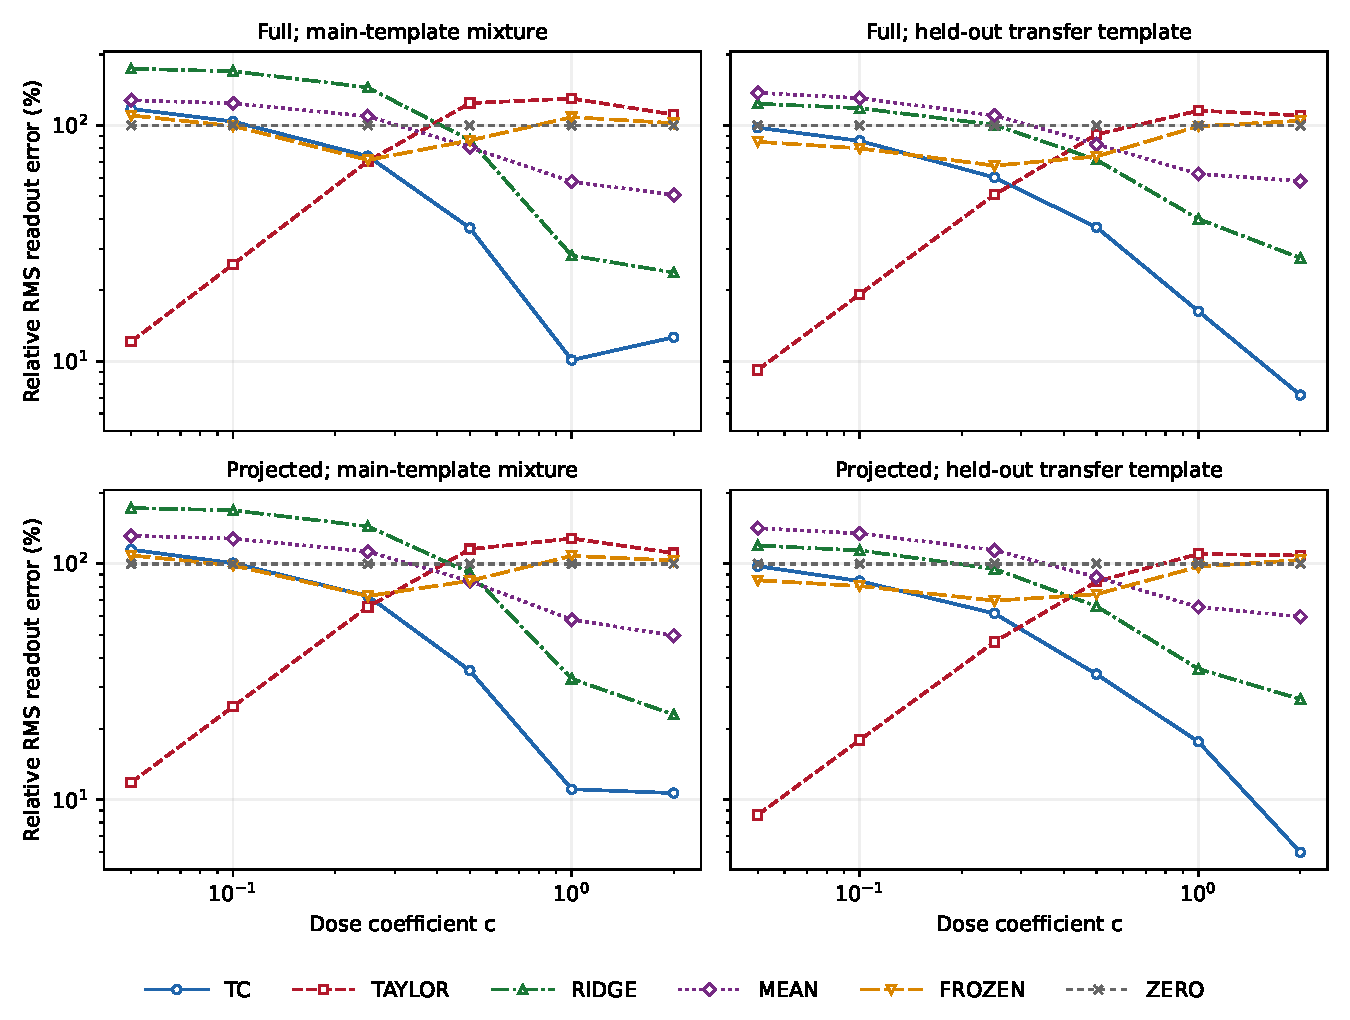
\includegraphics[width=\linewidth]{figures/new_test_dose.pdf}
\caption{All six Gemma-270M TEST doses, main mixture and transfer. Points are descriptive pooled relative RMS errors; line styles and markers distinguish predictors. Lines connect measured doses. Full numerical grids and interval scopes are in the supplement.}\label{fig:dose}
\end{figure}

\subsection{Gemma-1B: the crossover repeats, full-patch usefulness does not}
The second artifact repeats Taylor's small-dose advantage and larger-dose disadvantage, but its full-patch TC error exceeds zero change, ridge and the FIT class mean (Table~\ref{tab:second}). At dose 2, TC beats zero and mean while still losing to ridge. Thus crossover and useful accuracy are empirically separable.

\begin{table}[ht]\centering\small
\begin{tabular}{lrrrrr}\toprule Condition & TC & Taylor & Ridge & Mean & Zero\\\midrule
Main, $c=.05$ & 134.18 & 23.56 & 84.78 & 94.91 & 100\\
Main, $c=1$ & 115.38 & 269.86 & 50.80 & 66.99 & 100\\
Main, $c=2$ & 41.86 & 110.86 & 34.63 & 43.73 & 100\\
Transfer, $c=1$ & 137.43 & 267.26 & 60.81 & --- & 100\\\bottomrule\end{tabular}
\caption{Gemma-1B relative RMS error, percent, on 256 further blocks. All 144 metric cells, including the omitted compact-display mean, are in the supplement. Fixed-fit nominal intervals apply only as reported for this follow-up.}\label{tab:second}
\end{table}

At the full patch, TC absolute RMS is .4406 logits, Taylor 1.0306 and ridge .1940; native signal RMS is .3819. The TC relative-RMS nominal interval is [112.72\%,118.25\%], conditional on FIT. Transfer TC error also exceeds frozen-mask error, 127.55\%. Figure~\ref{fig:second} retains every dose and separates absolute from relative behavior.

\begin{figure}[ht]\centering
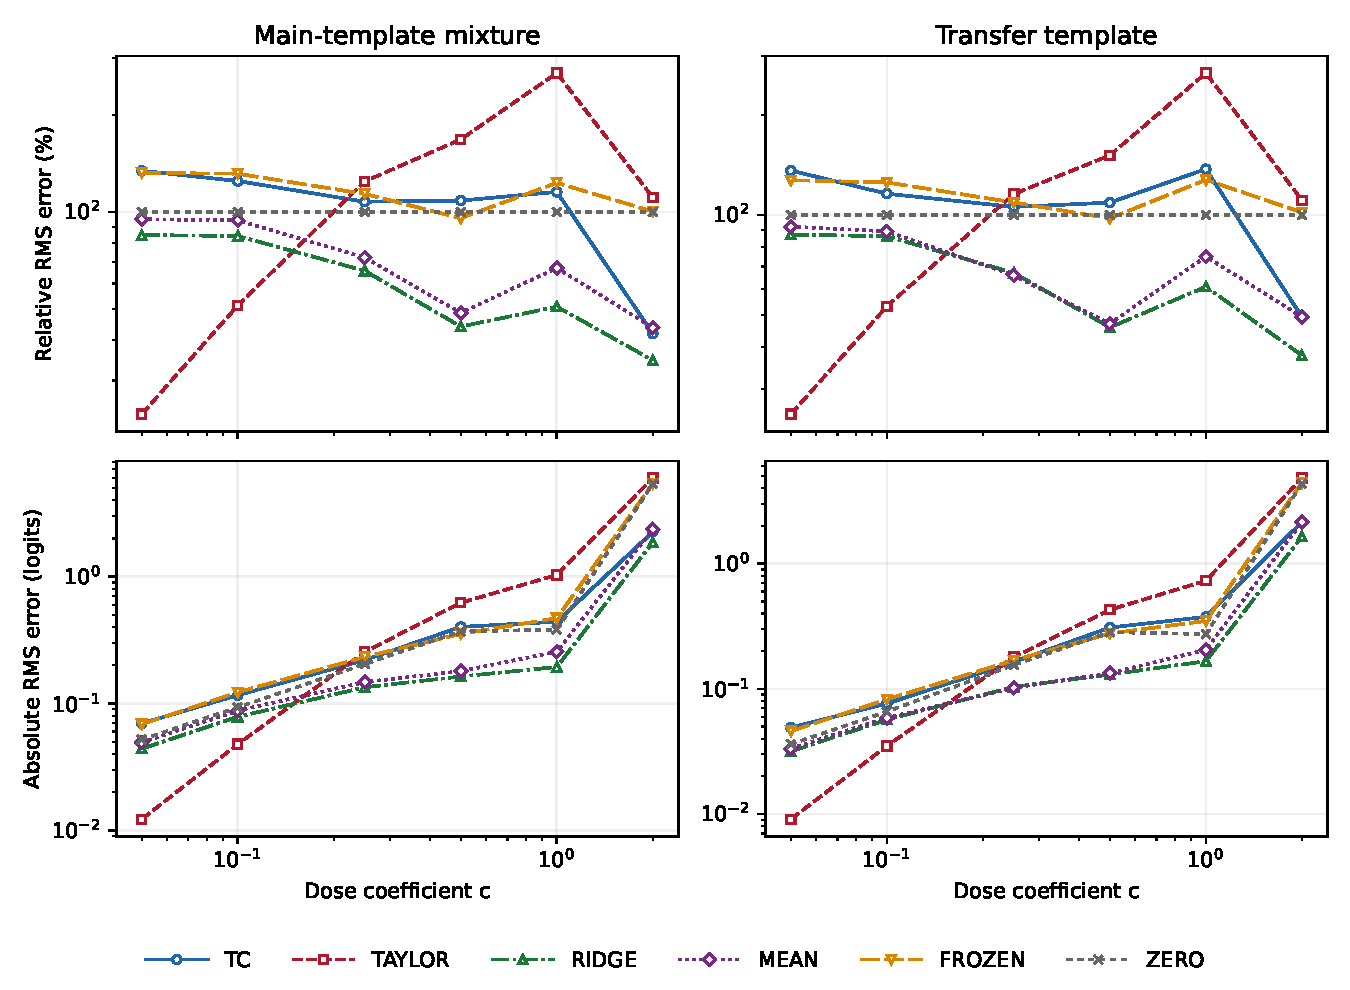
\includegraphics[width=\linewidth]{figures/second_artifact_dose.pdf}
\caption{Second-artifact dose curve. Relative and absolute method rankings agree within each condition. Shared templates retain the same lexical-block dependence. The full-patch failure and the still-stronger ridge comparator remain visible.}\label{fig:second}
\end{figure}

\section{Residual geometry and controlled prediction diagnostics}
\subsection{Endpoint cancellation is a vector observation}
With endpoint reconstruction errors $e_0=T(z)-f(z)$ and $e_1=T(z+\delta)-f(z+\delta)$, the TC delta error is $e_1-e_0$. Its energy is
\[
 \mathbb E\|e_1-e_0\|^2=\mathbb E\|e_1\|^2+\mathbb E\|e_0\|^2-2\mathbb E(e_1^\top e_0).
\]
At a full donor swap the endpoint-energy distributions are equal by the paired construction. In the complete 256-block cache, all-three-template pooled endpoint energy is $1.359397\times10^6$ at each endpoint, versus delta-error energy $.706683\times10^6$. The mixed term combines a mean component $-.859141\times10^6$ and centered component $-1.152970\times10^6$.

Centering changes the interpretation: within so/when/transfer the centered components are positive ($+.028933,+.019382,+.026141$, in $10^6$ units), while their across-frame pooled counterpart is negative. Between-frame offsets drive that sign change. This exact decomposition characterizes vector differences; the suffix separately determines readout accuracy.

Pooling all three templates, residual RMS grows from 95.31 to 840.64 between doses .05 and 1, and finite readout-error RMS from .05422 to .34459 logits. The natural-point gradient terms are .05578/.26671 and remainder RMS .00539/.12742. The growing absolute error and appreciable full-dose remainder constrain a local-gradient explanation. Supplementary tables retain each frame/operator/dose and the centering identities.

\subsection{Same-dose residual direction and selected mask changes}
Two posthoc experiments use 32 exposed blocks (indices 16--47), three frames, two sides, both operators and doses .05/1: 768 conditions. For native target $n_i$, TC prediction $t_i$ and residual $r_i=t_i-n_i$, the whole-residual substitution is
\[
 n_i+\|r_i\|r_j/\|r_j\|,
\]
using cyclic partner shifts 1 and 7 within each frame/side/operator/dose. This oracle construction preserves the original residual norm up to checked FP32 rounding. It adds no dose-independent endpoint-baseline mismatch.

At full dose/full edits, original pooled MSE is .11153 versus .14940/.18659 under the two substitutions; projected values are .12119 versus .23641/.25200. Every full-dose frame favors the original direction. The small-dose transfer/full partner7 contrast instead improves loss by .0001594. Both outcomes and all strata are retained.

For the mask experiment, write endpoint preactivations $a_0,a_1$, masks $m_0,m_1$ and $u_1=\operatorname{ReLU}(a_1)$. The endpoint code is decomposed as $h_{base}=u_1m_0$ plus switch contribution $s=u_1(m_1-m_0)$. ONLY allows $1_Gs$; EXCEPT allows $(1-1_G)s$. Original decoder/bias, endpoint magnitudes and nonswitching contributions remain. FIT scores select top32; a fixed random32 group is drawn from its complement.

At full dose/full edits, ONLY-top MSE .10463 is close to original .11153; EXCEPT-top gives 8.93294. Projected values are .11782/7.45841 versus .12119 original. At small dose, removing top32 slightly improves pooled loss. Random groups switch much less: .02083 features versus 8.3125 for top32, with no switches in 188/192 full contexts and 191/192 projected contexts. The selected-versus-random contrast therefore includes a large difference in actual intervention strength.

\subsection{Failed unscaled matching and a fresh fixed-norm direction contrast}
A cached FIT audit uses 32 blocks, 128 documents. Five fixed size-32 alternatives disjoint from top32 have mean switch counts 6.05--6.19 versus 10.375 and norms 211.47--222.38 versus 747.39. A triangle-inequality certificate bounds the mean norm of any such disjoint size-32 group by 441.559. Its implied norm-distribution Wasserstein-1 distance is at least 305.828, above the frozen descriptive FIT band 207.058. Unscaled strength matching fails on this finite FIT support.

A separately reviewed diagnostic changes the operation to equal-vector-norm prediction directions:
\[
 y_G=y_{\mathrm{TC\_FULL}}-\rho S_G/\|S_G\|,
 \qquad \rho=101.51097375005,
\]
where $S_G$ is the summed signed threshold-switch decoder contribution. The six groups and scale are fixed from FIT; joint eligibility caps amplification at four. For each block, the primary contrast compares top32's MSE increment from TC\_FULL with the equal mean of five fixed alternative increments (Table~\ref{tab:norm}).

\begin{table}[ht]\centering\small
\begin{tabular}{lrrr}\toprule Cohort/frame & Eligible contexts & Blocks & Top minus controls\\\midrule
Exposed so/when & 128/128 & 32/32 & .165807\\
Fresh lexical so/when & 128/128 & 32/32 & .198352\\
Fresh changed context & 45/64 & 26/32 & .083652\\
Fresh object/readout & 12/64 & 9/32 & .013883\\\bottomrule\end{tabular}
\caption{Full-dose fixed-norm prediction-direction diagnostic, squared-logit MSE-increment units. Positive contrast means greater damage from removing top32's direction. Fresh estimates descriptively reproduce the contrast; no prespecified inferential decision or interval is attached. Coverage conditions on all six groups.}\label{tab:norm}
\end{table}

Fresh so/when data use the same artifact/readout, groups and scale on 32 disjoint lexical blocks. Changed context retains she/he. The object frame changes both construction and readout to her/him; its 12/64 contexts across nine blocks sharply restrict transfer coverage. These are interventions on TC predictions around TC\_FULL, scored through the native suffix.

The five alternatives share 28--31 features and yield one to four distinct directions per eligible context. Cache reconstruction verifies identical active coefficients and FP32 targets behind duplicate table entries; top32 is distinct throughout. The frozen mean gives each unique control direction weight equal to its multiplicity divided by five. Complete per-frame uniqueness counts and every group estimate are in the supplement. Blocks supply the sampling unit.

If $e=m_{\mathrm{TC\_FULL}}-m_N$ and $\Delta m=m_G-m_{\mathrm{TC\_FULL}}$, the exact MSE increment is
\[
 (e+\Delta m)^2-e^2=(\Delta m)^2+2e\Delta m.
\]
Readout sensitivity and alignment with existing signed error both matter. Approximate top32/TC-delta collinearity remains an untested hypothesis. Gradients at TC\_FULL have not been measured in these follow-ups; the supplement distinguishes earlier gradients at natural and native endpoints.

\section{A negative boundary on the Qwen component}
A separate extension evaluates the public Qwen3-0.6B-Base source27--target27 CLT component through final native normalization/head for is/are. It uses the companion repair study's 256 lexical blocks and two frames, adopting unit-dose native/first-fit ridge outputs. Other-dose FIT comparators and CLT/frozen/Taylor predictions follow a separate frozen protocol. Table~\ref{tab:qwen} records the resulting boundary.

\begin{table}[ht]\centering\small
\begin{tabular}{lrr}\toprule Predictor & Main $c=.05$ & Main $c=1$\\\midrule
CLT component & 99.830 & 100.347\\
Native-vector Taylor & 3.172 & 34.600\\
Composed scalar linear & 3.305 & 35.904\\
Frozen recipient mask & 99.830 & 100.302\\
FIT ridge & 36.499 & 30.572\\
FIT conditional mean & 37.589 & 37.757\\
Zero change & 100.000 & 100.000\\\bottomrule\end{tabular}
\caption{Qwen component relative RMS error, percent. Descriptive shared-cohort extension; all six doses and both frames are in the supplement. The CLT component remains near the zero-change baseline.}\label{tab:qwen}
\end{table}

At full dose, absolute CLT error is 2.45515 logits, versus .84654 for Taylor and .74800 for ridge; native signal RMS is 2.44665. Frame-specific CLT relative errors are 100.022\%/100.625\%. This extension therefore supplies no Gemma-like useful regime. The tested normalized-input operator passed separate hook/head/JVP/reachability checks. Exact adoption mappings distinguish the 128-label first-fit ridge here from the companion's Direct256 predictor.

\section{Limitations and interpretation}
The positive result is conditional on a selected public artifact, branch, synthetic pronoun task and two-token readout. The fresh lexical protocol tests that setting prospectively, while the second-artifact and Qwen results bound transfer. Artifact, model, layer, suffix and readout change together across comparisons. The evidence therefore supports artifact-specific usefulness rather than an isolated model-family or scale explanation.

The mechanism diagnostics have distinct interventions and access. Whole-residual substitution needs oracle native targets; mask and fixed-norm directions use TC activations. Selected-mask preservation keeps other features and endpoint magnitudes. Equal norm leaves switch count, basis content and curvature unequal; duplicate control multiplicities remain part of the frozen estimand. Exposed-data analyses, fresh eligible subsets and earlier cyclic endpoint-baseline substitutions keep their separate scopes. The earlier 16-block construction adds a dose-independent baseline-error mismatch and shows operator-dependent effects; complete negative strata and interactions remain in the supplement.

Relative error measures prediction of an intervention's margin effect. Its denominator is native signal energy; general answer quality and full replacement-circuit fidelity require other outcomes. The first artifact's absolute error increases with dose, and pooled vector cancellation depends on centering. Neither observation by itself establishes a causal explanation of the favorable full-patch regime. The current directions and endpoint gradients leave TC\_FULL alignment and gradient hypotheses open.

Inference is similarly scoped: the original hypothesis family remains unqualified; the qualified 270M interval family, nominal 1B intervals and descriptive direction follow-ups retain their own limits. Public-TC and native-FIT resource budgets are unequal. Complete operation accounting, failed starts, cache aliases and independent reviews are in the supplement and source bundle. Authorship, public evidence location and licensing/release disclosures require completion before submission.

The empirical conclusion is a dose-dependent separation of local response fidelity, finite-effect usefulness and ranking against Taylor. Gemma-270M demonstrates useful full-patch prediction; Gemma-1B repeats crossover with poor full-patch accuracy; the Qwen component provides a negative boundary. The controlled diagnostics narrow the geometry of the first success while leaving a complete mechanism open.

\clearpage
\small
\bibliographystyle{plain}
\bibliography{references}
\end{document}
